\documentclass[12pt]{article}
\usepackage{amsmath,amssymb,amsthm}
\usepackage{graphicx,mathabx}
\usepackage{xcolor}
\usepackage{tikz}
\usepackage{placeins}
\usepackage{lipsum}
\usepackage[shortlabels]{enumitem}
\usepackage{placeins}
\usepackage[makeroom]{cancel}
\usepackage[strings]{underscore} 
\usepackage{afterpage}
\newcommand\tab[1][1cm]{\hspace*{#1}}
\newcommand\blankpage{%
    \null
    \thispagestyle{empty}%
    \addtocounter{page}{-1}%
    \newpage}
\begin{document}
\title{TCSS 343 - Week 6}
\author{Jake McKenzie}
\maketitle
\noindent\centerline{\textbf{More problems in Dynamic Programming and Greedy Algoritms}}\\\\\\\\\\\\
\begin{center}
    ``A distributed system is when some computer I don't know about fails and causes my computer to fail." \\$\dots$\\ Leslie Lamport
\end{center}
\begin{center}
    ``Pain is inevitable, suffering is optional." \\$\dots$\\ Haruki Murakami
\end{center}
\newpage
\noindent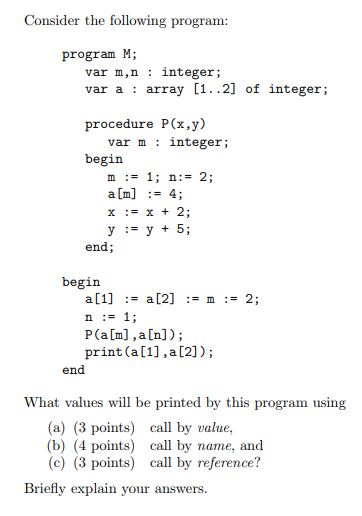
\includegraphics[scale = 1]{debugging.JPG}
\newpage
\noindent Prove that if $n \in \mathbb{Z}$ and $5n+4$ is even, then $n$ is even using proof by contradiction.
(\textbf{Motivation: }Proof by contradiction is often used in proving greedy algorithms correct.)
\newpage
\noindent In mathematics, a sequence of positive real numbers 
$s_1$, $s_2$,$\dots$ is called \textit{superincreasing} if each element
in the sequence is greater than the sum of all previous elements in the sequence:
$$s_{n+1} > \sum\limits_{i=1}^{n}s_i$$
For example: \{$2,3,7,16,65,321,4546$\} is a superincreasing sequence, 
but \{$1,1,2,5,15,52,203,877$\} us not a superincreasing sequence.\\\\
Describe an algorithm that takes as input superincreasing sequence $s_1,\dots,s_n$ and a positive 
integer $k$, please find a sequnce of $s_1,\dots,s_n$ with the sum equal
to $k$. It is possible and desirable to find an algorithm that can accomplish this
task in $O(n)$ time using dynamic progrmaming. If you think you've come up with an
algorithm that can accomplish this task attempt to prove that it is correct.
\newpage
\noindent \textbf{The Knapsack Problem: }Given an integer $K$ and $n$ items of different sizes such 
that the $i^{th}$ item has an integer size of $k_i$, find a subset of the items whose sizes sum 
to exactly K, or determin no such subset exists.\\\\
\textbf{Knapsack(S,K):}\\\\
\textbf{Input: }S(an array of size n storing the sizes of the items)\\\\
\textbf{Output: }P(a two dimensional array such that P[i,k].exist() = true if there 
exists a solution to the knapsack problem with the first i elements and a knapsack of size 
k, and P[i,k].belong = true if the $i^{th}$ element belongs to the solution)\\\\
Give an algorithm that solves this problem given these input and output parameters. 
\end{document}